\documentclass[twoside]{book}

% Packages required by doxygen
\usepackage{fixltx2e}
\usepackage{calc}
\usepackage{doxygen}
\usepackage[export]{adjustbox} % also loads graphicx
\usepackage{graphicx}
\usepackage[utf8]{inputenc}
\usepackage{makeidx}
\usepackage{multicol}
\usepackage{multirow}
\PassOptionsToPackage{warn}{textcomp}
\usepackage{textcomp}
\usepackage[nointegrals]{wasysym}
\usepackage[table]{xcolor}

% NLS support packages
\usepackage[T2A]{fontenc}
\usepackage[russian]{babel}

% Font selection
\usepackage[T1]{fontenc}
\usepackage[scaled=.90]{helvet}
\usepackage{courier}
\usepackage{amssymb}
\usepackage{sectsty}
\renewcommand{\familydefault}{\sfdefault}
\allsectionsfont{%
  \fontseries{bc}\selectfont%
  \color{darkgray}%
}
\renewcommand{\DoxyLabelFont}{%
  \fontseries{bc}\selectfont%
  \color{darkgray}%
}
\newcommand{\+}{\discretionary{\mbox{\scriptsize$\hookleftarrow$}}{}{}}

% Page & text layout
\usepackage{geometry}
\geometry{%
  a4paper,%
  top=2.5cm,%
  bottom=2.5cm,%
  left=2.5cm,%
  right=2.5cm%
}
\tolerance=750
\hfuzz=15pt
\hbadness=750
\setlength{\emergencystretch}{15pt}
\setlength{\parindent}{0cm}
\setlength{\parskip}{3ex plus 2ex minus 2ex}
\makeatletter
\renewcommand{\paragraph}{%
  \@startsection{paragraph}{4}{0ex}{-1.0ex}{1.0ex}{%
    \normalfont\normalsize\bfseries\SS@parafont%
  }%
}
\renewcommand{\subparagraph}{%
  \@startsection{subparagraph}{5}{0ex}{-1.0ex}{1.0ex}{%
    \normalfont\normalsize\bfseries\SS@subparafont%
  }%
}
\makeatother

% Headers & footers
\usepackage{fancyhdr}
\pagestyle{fancyplain}
\fancyhead[LE]{\fancyplain{}{\bfseries\thepage}}
\fancyhead[CE]{\fancyplain{}{}}
\fancyhead[RE]{\fancyplain{}{\bfseries\leftmark}}
\fancyhead[LO]{\fancyplain{}{\bfseries\rightmark}}
\fancyhead[CO]{\fancyplain{}{}}
\fancyhead[RO]{\fancyplain{}{\bfseries\thepage}}
\fancyfoot[LE]{\fancyplain{}{}}
\fancyfoot[CE]{\fancyplain{}{}}
\fancyfoot[RE]{\fancyplain{}{\bfseries\scriptsize Создано системой Doxygen }}
\fancyfoot[LO]{\fancyplain{}{\bfseries\scriptsize Создано системой Doxygen }}
\fancyfoot[CO]{\fancyplain{}{}}
\fancyfoot[RO]{\fancyplain{}{}}
\renewcommand{\footrulewidth}{0.4pt}
\renewcommand{\chaptermark}[1]{%
  \markboth{#1}{}%
}
\renewcommand{\sectionmark}[1]{%
  \markright{\thesection\ #1}%
}

% Indices & bibliography
\usepackage{natbib}
\usepackage[titles]{tocloft}
\setcounter{tocdepth}{3}
\setcounter{secnumdepth}{5}
\makeindex

% Hyperlinks (required, but should be loaded last)
\usepackage{ifpdf}
\ifpdf
  \usepackage[pdftex,pagebackref=true]{hyperref}
\else
  \usepackage[ps2pdf,pagebackref=true]{hyperref}
\fi
\hypersetup{%
  colorlinks=true,%
  linkcolor=blue,%
  citecolor=blue,%
  unicode%
}

% Custom commands
\newcommand{\clearemptydoublepage}{%
  \newpage{\pagestyle{empty}\cleardoublepage}%
}

\usepackage{caption}
\captionsetup{labelsep=space,justification=centering,font={bf},singlelinecheck=off,skip=4pt,position=top}

%===== C O N T E N T S =====

\begin{document}

% Titlepage & ToC
\hypersetup{pageanchor=false,
             bookmarksnumbered=true,
             pdfencoding=unicode
            }
\pagenumbering{alph}
\begin{titlepage}
\vspace*{7cm}
\begin{center}%
{\Large My Project }\\
\vspace*{1cm}
{\large Создано системой Doxygen 1.8.13}\\
\end{center}
\end{titlepage}
\clearemptydoublepage
\pagenumbering{roman}
\tableofcontents
\clearemptydoublepage
\pagenumbering{arabic}
\hypersetup{pageanchor=true}

%--- Begin generated contents ---
\chapter{Иерархический список классов}
\section{Иерархия классов}
Иерархия классов.\begin{DoxyCompactList}
\item invalid\+\_\+argument\begin{DoxyCompactList}
\item \contentsline{section}{cipher\+\_\+error}{\pageref{classcipher__error}}{}
\end{DoxyCompactList}
\item \contentsline{section}{mod\+Alpha\+Cipher}{\pageref{classmodAlphaCipher}}{}
\end{DoxyCompactList}

\chapter{Алфавитный указатель классов}
\section{Классы}
Классы с их кратким описанием.\begin{DoxyCompactList}
\item\contentsline{section}{\hyperlink{classcipher__error}{cipher\+\_\+error} }{\pageref{classcipher__error}}{}
\item\contentsline{section}{\hyperlink{classmodAlphaCipher}{mod\+Alpha\+Cipher} \\*Шифрование методом Гронсфельда }{\pageref{classmodAlphaCipher}}{}
\end{DoxyCompactList}

\chapter{Список файлов}
\section{Файлы}
Полный список документированных файлов.\begin{DoxyCompactList}
\item\contentsline{section}{\hyperlink{main_8cpp}{main.\+cpp} \\*Главный файл для модуля swapcipher }{\pageref{main_8cpp}}{}
\item\contentsline{section}{\hyperlink{swapcipher_8cpp}{swapcipher.\+cpp} \\*Исполняемый файл для модуля swapcipher }{\pageref{swapcipher_8cpp}}{}
\item\contentsline{section}{\hyperlink{swapcipher_8h}{swapcipher.\+h} \\*Заголовочный файл для модуля swapcipher }{\pageref{swapcipher_8h}}{}
\end{DoxyCompactList}

\chapter{Классы}
\hypertarget{classcipher__error}{}\section{Класс cipher\+\_\+error}
\label{classcipher__error}\index{cipher\+\_\+error@{cipher\+\_\+error}}


Граф наследования\+:cipher\+\_\+error\+:\nopagebreak
\begin{figure}[H]
\begin{center}
\leavevmode
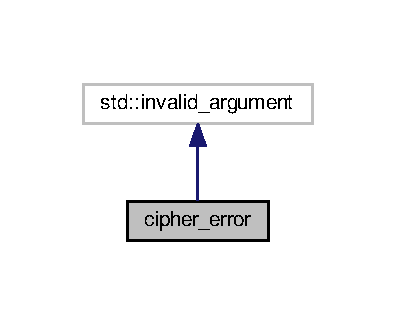
\includegraphics[width=190pt]{classcipher__error__inherit__graph}
\end{center}
\end{figure}


Граф связей класса cipher\+\_\+error\+:\nopagebreak
\begin{figure}[H]
\begin{center}
\leavevmode
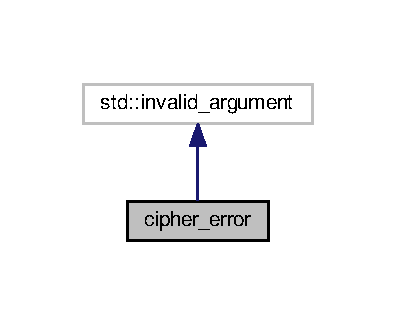
\includegraphics[width=190pt]{classcipher__error__coll__graph}
\end{center}
\end{figure}
\subsection*{Открытые члены}
\begin{DoxyCompactItemize}
\item 
\mbox{\Hypertarget{classcipher__error_aac662e216a84bfeb873303c7b88d029e}\label{classcipher__error_aac662e216a84bfeb873303c7b88d029e}} 
{\bfseries cipher\+\_\+error} (const std\+::string \&what\+\_\+arg)
\item 
\mbox{\Hypertarget{classcipher__error_a18cf27d9c2cd2538d3cb8f17e9a55f3e}\label{classcipher__error_a18cf27d9c2cd2538d3cb8f17e9a55f3e}} 
{\bfseries cipher\+\_\+error} (const char $\ast$what\+\_\+arg)
\end{DoxyCompactItemize}


Объявления и описания членов класса находятся в файле\+:\begin{DoxyCompactItemize}
\item 
\hyperlink{modAlphaCipher_8h}{mod\+Alpha\+Cipher.\+h}\end{DoxyCompactItemize}

\hypertarget{classmodAlphaCipher}{}\section{Класс mod\+Alpha\+Cipher}
\label{classmodAlphaCipher}\index{mod\+Alpha\+Cipher@{mod\+Alpha\+Cipher}}


Шифрование методом Гронсфельда  




{\ttfamily \#include $<$mod\+Alpha\+Cipher.\+h$>$}

\subsection*{Открытые члены}
\begin{DoxyCompactItemize}
\item 
\mbox{\Hypertarget{classmodAlphaCipher_a76a420025b3c08f72c9b996d83c6ff09}\label{classmodAlphaCipher_a76a420025b3c08f72c9b996d83c6ff09}} 
{\bfseries mod\+Alpha\+Cipher} (const std\+::string \&skey)
\item 
std\+::string \hyperlink{classmodAlphaCipher_ab855d6b2ba63a70d84abc8b15700da63}{encrypt} (const std\+::string \&open\+\_\+text)
\begin{DoxyCompactList}\small\item\em Зашифровывание \end{DoxyCompactList}\item 
\mbox{\Hypertarget{classmodAlphaCipher_af1f0fa8ec93df56aa7657494de2a3f00}\label{classmodAlphaCipher_af1f0fa8ec93df56aa7657494de2a3f00}} 
std\+::string {\bfseries decrypt} (const std\+::string \&cipher\+\_\+text)
\end{DoxyCompactItemize}
\subsection*{Закрытые члены}
\begin{DoxyCompactItemize}
\item 
\mbox{\Hypertarget{classmodAlphaCipher_ab8f9e5e8ee499c8df2d1e45822f5ac7f}\label{classmodAlphaCipher_ab8f9e5e8ee499c8df2d1e45822f5ac7f}} 
std\+::vector$<$ int $>$ {\bfseries convert} (const std\+::string \&s)
\item 
\mbox{\Hypertarget{classmodAlphaCipher_afa3ddac1b01e7847238478963d667d4a}\label{classmodAlphaCipher_afa3ddac1b01e7847238478963d667d4a}} 
std\+::string {\bfseries convert} (const std\+::vector$<$ int $>$ \&v)
\item 
\mbox{\Hypertarget{classmodAlphaCipher_a6e22f85d0847650a18be5838ca9175c5}\label{classmodAlphaCipher_a6e22f85d0847650a18be5838ca9175c5}} 
std\+::string {\bfseries get\+Valid\+Key} (const std\+::string \&s)
\item 
\mbox{\Hypertarget{classmodAlphaCipher_ace571c0bf1e21e6cb31f3df78a1812bd}\label{classmodAlphaCipher_ace571c0bf1e21e6cb31f3df78a1812bd}} 
std\+::string {\bfseries get\+Valid\+Open\+Text} (const std\+::string \&s)
\item 
\mbox{\Hypertarget{classmodAlphaCipher_a29591c14f56205ecad3d99689bf72193}\label{classmodAlphaCipher_a29591c14f56205ecad3d99689bf72193}} 
std\+::string {\bfseries get\+Valid\+Cipher\+Text} (const std\+::string \&s)
\end{DoxyCompactItemize}
\subsection*{Закрытые данные}
\begin{DoxyCompactItemize}
\item 
\mbox{\Hypertarget{classmodAlphaCipher_ab7e0c7d3c87f4c8b7435d84f31c6cb62}\label{classmodAlphaCipher_ab7e0c7d3c87f4c8b7435d84f31c6cb62}} 
std\+::wstring {\bfseries num\+Alpha} = L\char`\"{}АБВГДЕЁЖЗИЙКЛМНОПРСТУФХЦЧШЩЪЫЬЭЮЯ\char`\"{}
\item 
\mbox{\Hypertarget{classmodAlphaCipher_ad896cbfa7d4c32d1c9627b0812b4a677}\label{classmodAlphaCipher_ad896cbfa7d4c32d1c9627b0812b4a677}} 
std\+::map$<$ wchar\+\_\+t, int $>$ {\bfseries alpha\+Num}
\item 
\mbox{\Hypertarget{classmodAlphaCipher_aaddfb3bc0a3806b17e94c56fea5bad87}\label{classmodAlphaCipher_aaddfb3bc0a3806b17e94c56fea5bad87}} 
std\+::vector$<$ int $>$ \hyperlink{classmodAlphaCipher_aaddfb3bc0a3806b17e94c56fea5bad87}{key}
\begin{DoxyCompactList}\small\item\em ключ \end{DoxyCompactList}\end{DoxyCompactItemize}


\subsection{Подробное описание}
Шифрование методом Гронсфельда 

Ключ устанавливается в конструкторе. Для зашифровывания и расшифровывания предназначены методы encrypt и decrypt. \begin{DoxyWarning}{Предупреждения}
Реализация только для русского языка 
\end{DoxyWarning}


\subsection{Методы}
\mbox{\Hypertarget{classmodAlphaCipher_ab855d6b2ba63a70d84abc8b15700da63}\label{classmodAlphaCipher_ab855d6b2ba63a70d84abc8b15700da63}} 
\index{mod\+Alpha\+Cipher@{mod\+Alpha\+Cipher}!encrypt@{encrypt}}
\index{encrypt@{encrypt}!mod\+Alpha\+Cipher@{mod\+Alpha\+Cipher}}
\subsubsection{\texorpdfstring{encrypt()}{encrypt()}}
{\footnotesize\ttfamily std\+::string mod\+Alpha\+Cipher\+::encrypt (\begin{DoxyParamCaption}\item[{const std\+::string \&}]{open\+\_\+text }\end{DoxyParamCaption})}



Зашифровывание 


\begin{DoxyParams}[1]{Аргументы}
\mbox{\tt in}  & {\em open\+\_\+text} & Открытый текст. Не должен быть пустой строкой. Строчные символы автоматически преобразуются к прописным. Все не-\/буквы удаляются \\
\hline
\end{DoxyParams}
\begin{DoxyReturn}{Возвращает}
Зашифрованная строка 
\end{DoxyReturn}

\begin{DoxyExceptions}{Исключения}
{\em \hyperlink{classcipher__error}{cipher\+\_\+error},если} & текст пустой \\
\hline
\end{DoxyExceptions}


Объявления и описания членов классов находятся в файлах\+:\begin{DoxyCompactItemize}
\item 
\hyperlink{modAlphaCipher_8h}{mod\+Alpha\+Cipher.\+h}\item 
mod\+Alpha\+Cipher.\+cpp\end{DoxyCompactItemize}

\chapter{Файлы}
\hypertarget{modAlphaCipher_8h}{}\section{Файл mod\+Alpha\+Cipher.\+h}
\label{modAlphaCipher_8h}\index{mod\+Alpha\+Cipher.\+h@{mod\+Alpha\+Cipher.\+h}}


Заголовочный файл для модуля Gronsfeld.  


{\ttfamily \#include $<$vector$>$}\newline
{\ttfamily \#include $<$string$>$}\newline
{\ttfamily \#include $<$map$>$}\newline
Граф включаемых заголовочных файлов для mod\+Alpha\+Cipher.\+h\+:\nopagebreak
\begin{figure}[H]
\begin{center}
\leavevmode
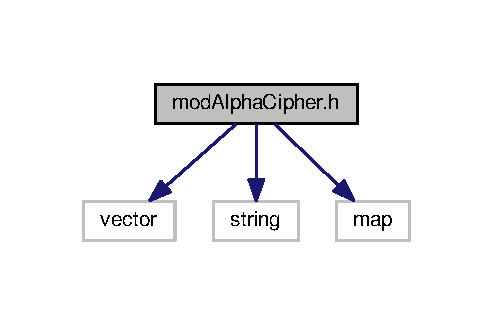
\includegraphics[width=237pt]{modAlphaCipher_8h__incl}
\end{center}
\end{figure}
\subsection*{Классы}
\begin{DoxyCompactItemize}
\item 
class \hyperlink{classmodAlphaCipher}{mod\+Alpha\+Cipher}
\begin{DoxyCompactList}\small\item\em Шифрование методом Гронсфельда \end{DoxyCompactList}\item 
class \hyperlink{classcipher__error}{cipher\+\_\+error}
\end{DoxyCompactItemize}


\subsection{Подробное описание}
Заголовочный файл для модуля Gronsfeld. 

\begin{DoxyAuthor}{Автор}
Григорьев А.\+Д. 
\end{DoxyAuthor}
\begin{DoxyVersion}{Версия}
1.\+0 
\end{DoxyVersion}
\begin{DoxyDate}{Дата}
09.\+06.\+2019 
\end{DoxyDate}
\begin{DoxyCopyright}{Авторство}
ИБСТ ПГУ 
\end{DoxyCopyright}
\begin{DoxyWarning}{Предупреждения}
Это учебный пример 
\end{DoxyWarning}

%--- End generated contents ---

% Index
\backmatter
\newpage
\phantomsection
\clearemptydoublepage
\addcontentsline{toc}{chapter}{Алфавитный указатель}
\printindex

\end{document}
